
\begin{figure}[H]
  {
    \setlength{\tabcolsep}{3.0pt}
    \setlength\cmidrulewidth{\heavyrulewidth} % Make cmidrule = 
    \begin{adjustbox}{width=3cm,center}
      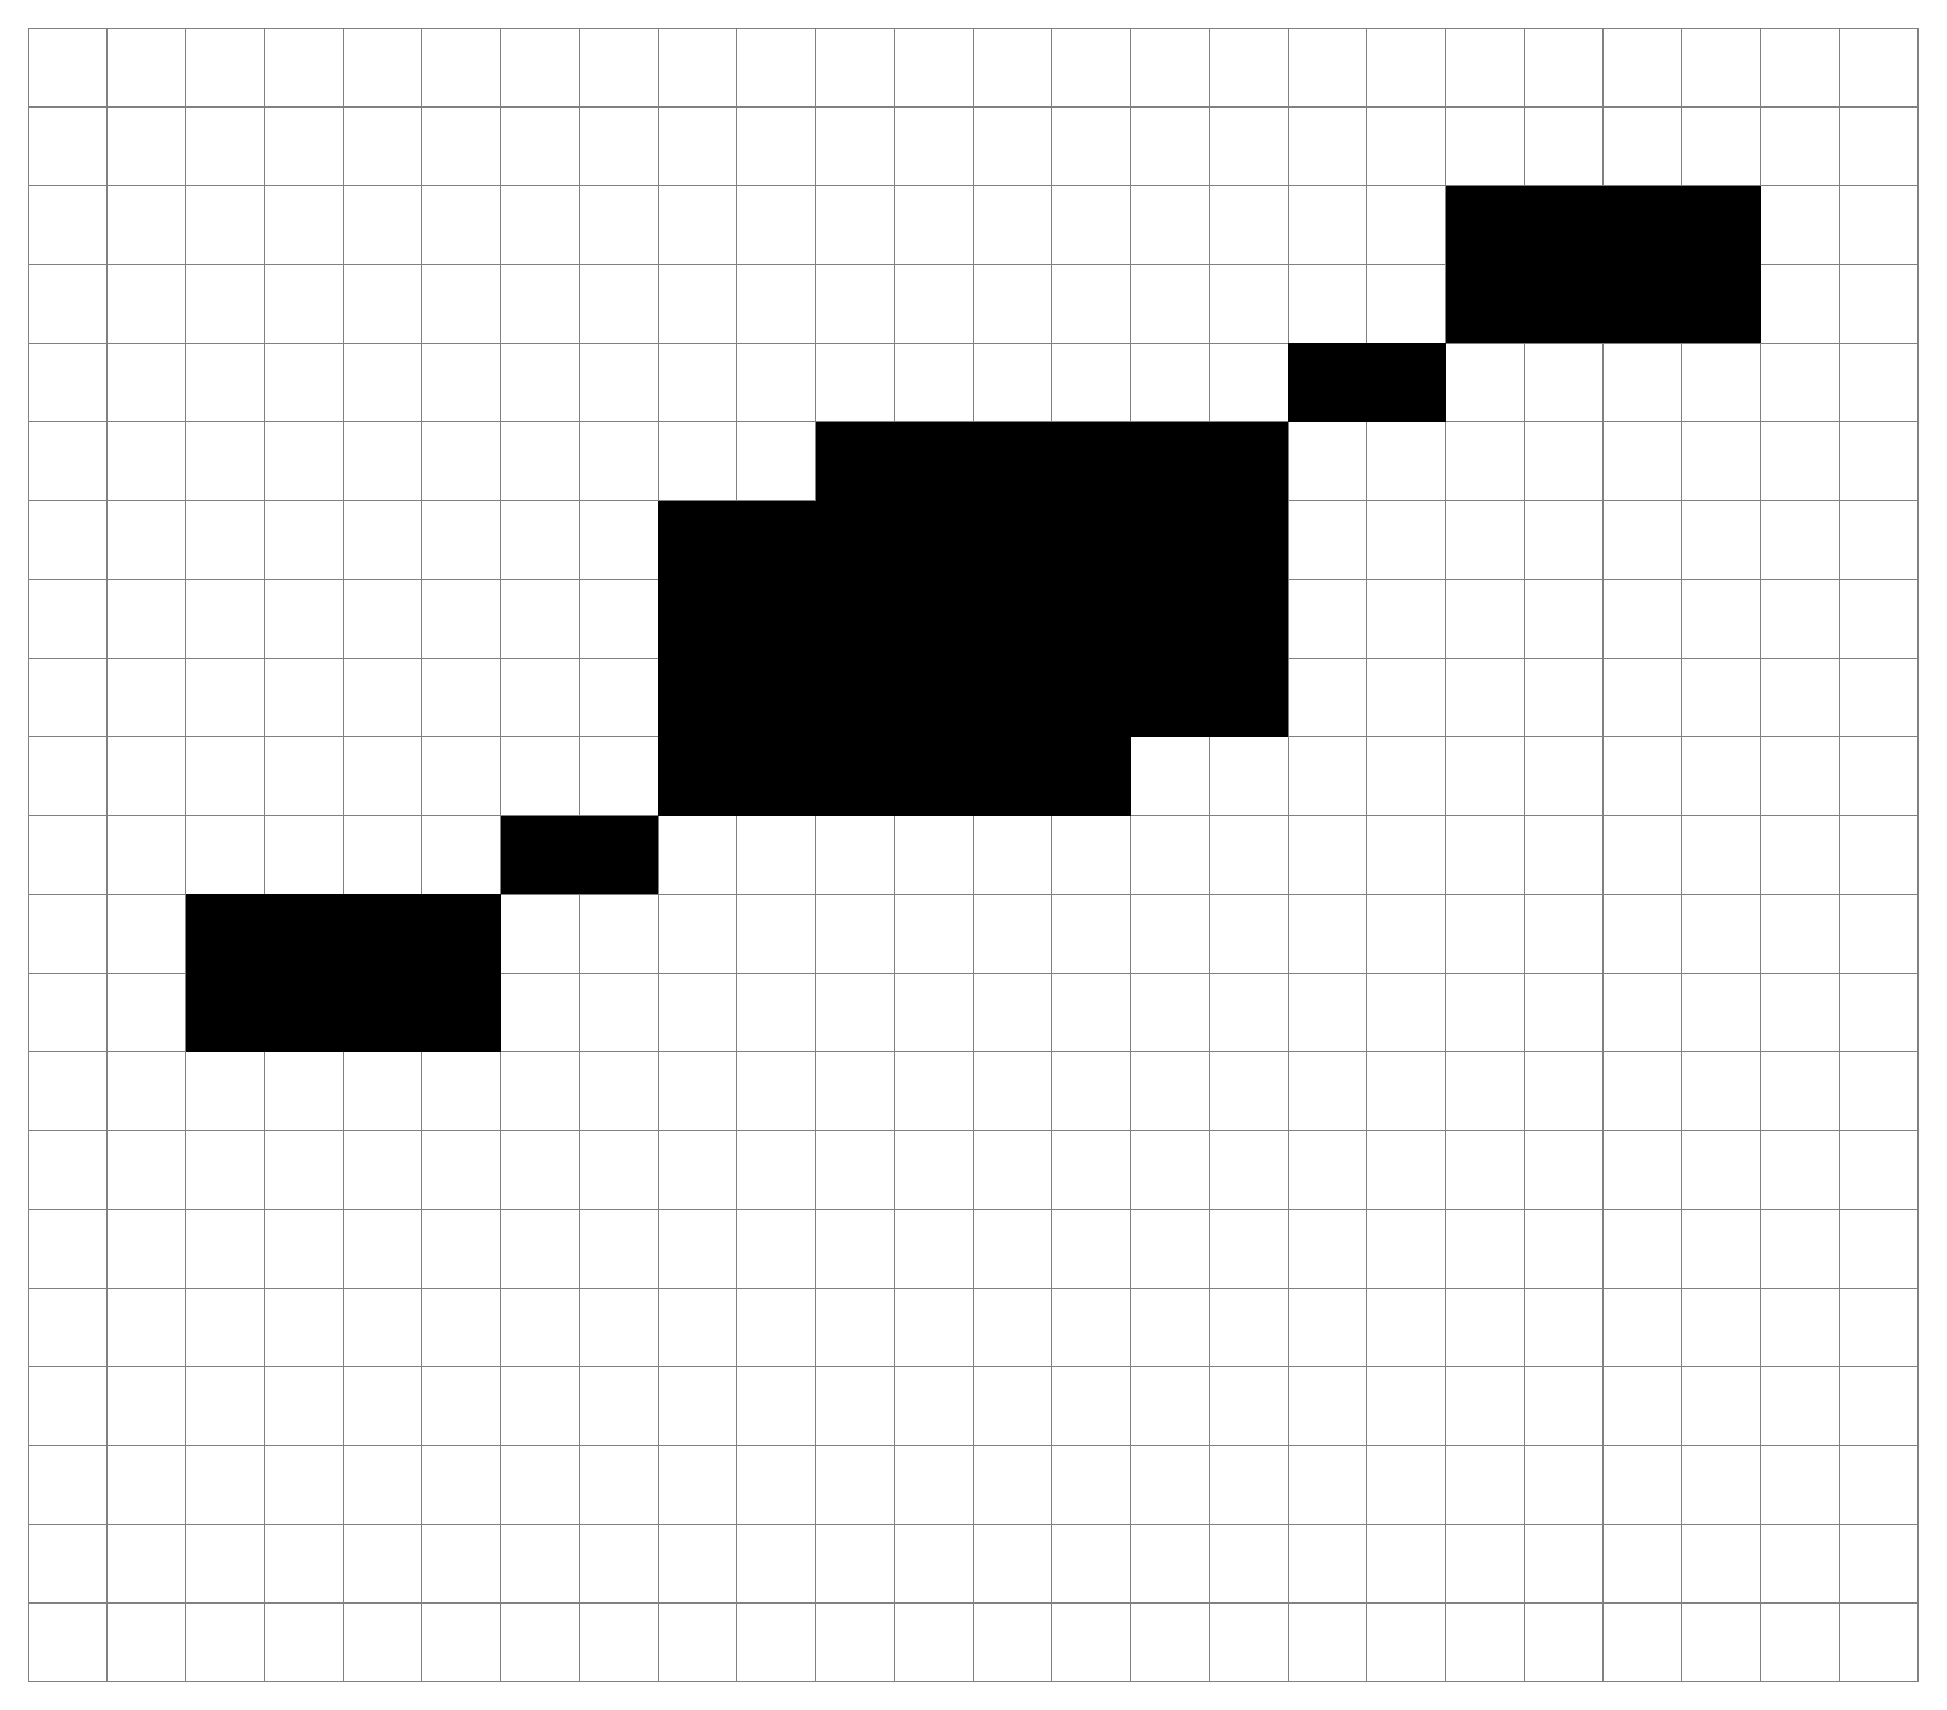
\begin{tikzpicture}

	\draw[step=1.0,gray,thin] (0,0) grid (24,21);
	\fill[\SPRITECOLOR] (18,18) rectangle ++ (1,1);
	\fill[\SPRITECOLOR] (19,18) rectangle ++ (1,1);
	\fill[\SPRITECOLOR] (20,18) rectangle ++ (1,1);
	\fill[\SPRITECOLOR] (21,18) rectangle ++ (1,1);
	\fill[\MULTICOLORONE] (18,17) rectangle ++ (1,1);
	\fill[\MULTICOLORONE] (19,17) rectangle ++ (1,1);
	\fill[\SPRITECOLOR] (20,17) rectangle ++ (1,1);
	\fill[\SPRITECOLOR] (21,17) rectangle ++ (1,1);
	\fill[\MULTICOLORONE] (16,16) rectangle ++ (1,1);
	\fill[\MULTICOLORONE] (17,16) rectangle ++ (1,1);
	\fill[\MULTICOLORTWO] (10,15) rectangle ++ (1,1);
	\fill[\MULTICOLORTWO] (11,15) rectangle ++ (1,1);
	\fill[\SPRITECOLOR] (12,15) rectangle ++ (1,1);
	\fill[\SPRITECOLOR] (13,15) rectangle ++ (1,1);
	\fill[\MULTICOLORONE] (14,15) rectangle ++ (1,1);
	\fill[\MULTICOLORONE] (15,15) rectangle ++ (1,1);
	\fill[\MULTICOLORTWO] (8,14) rectangle ++ (1,1);
	\fill[\MULTICOLORTWO] (9,14) rectangle ++ (1,1);
	\fill[\SPRITECOLOR] (10,14) rectangle ++ (1,1);
	\fill[\SPRITECOLOR] (11,14) rectangle ++ (1,1);
	\fill[\SPRITECOLOR] (12,14) rectangle ++ (1,1);
	\fill[\SPRITECOLOR] (13,14) rectangle ++ (1,1);
	\fill[\SPRITECOLOR] (14,14) rectangle ++ (1,1);
	\fill[\SPRITECOLOR] (15,14) rectangle ++ (1,1);
	\fill[\SPRITECOLOR] (8,13) rectangle ++ (1,1);
	\fill[\SPRITECOLOR] (9,13) rectangle ++ (1,1);
	\fill[\SPRITECOLOR] (10,13) rectangle ++ (1,1);
	\fill[\SPRITECOLOR] (11,13) rectangle ++ (1,1);
	\fill[\SPRITECOLOR] (12,13) rectangle ++ (1,1);
	\fill[\SPRITECOLOR] (13,13) rectangle ++ (1,1);
	\fill[\SPRITECOLOR] (14,13) rectangle ++ (1,1);
	\fill[\SPRITECOLOR] (15,13) rectangle ++ (1,1);
	\fill[\SPRITECOLOR] (8,12) rectangle ++ (1,1);
	\fill[\SPRITECOLOR] (9,12) rectangle ++ (1,1);
	\fill[\SPRITECOLOR] (10,12) rectangle ++ (1,1);
	\fill[\SPRITECOLOR] (11,12) rectangle ++ (1,1);
	\fill[\SPRITECOLOR] (12,12) rectangle ++ (1,1);
	\fill[\SPRITECOLOR] (13,12) rectangle ++ (1,1);
	\fill[\SPRITECOLOR] (14,12) rectangle ++ (1,1);
	\fill[\SPRITECOLOR] (15,12) rectangle ++ (1,1);
	\fill[\MULTICOLORONE] (8,11) rectangle ++ (1,1);
	\fill[\MULTICOLORONE] (9,11) rectangle ++ (1,1);
	\fill[\SPRITECOLOR] (10,11) rectangle ++ (1,1);
	\fill[\SPRITECOLOR] (11,11) rectangle ++ (1,1);
	\fill[\SPRITECOLOR] (12,11) rectangle ++ (1,1);
	\fill[\SPRITECOLOR] (13,11) rectangle ++ (1,1);
	\fill[\MULTICOLORONE] (6,10) rectangle ++ (1,1);
	\fill[\MULTICOLORONE] (7,10) rectangle ++ (1,1);
	\fill[\SPRITECOLOR] (2,9) rectangle ++ (1,1);
	\fill[\SPRITECOLOR] (3,9) rectangle ++ (1,1);
	\fill[\MULTICOLORONE] (4,9) rectangle ++ (1,1);
	\fill[\MULTICOLORONE] (5,9) rectangle ++ (1,1);
	\fill[\SPRITECOLOR] (2,8) rectangle ++ (1,1);
	\fill[\SPRITECOLOR] (3,8) rectangle ++ (1,1);
	\fill[\SPRITECOLOR] (4,8) rectangle ++ (1,1);
	\fill[\SPRITECOLOR] (5,8) rectangle ++ (1,1);

      \end{tikzpicture}
    \end{adjustbox}
  }\caption{BOLAS4}
\end{figure}
